\setcounter{section}{1}
\section{Pseudosolutions and its applications. Linear regression.}
\par 
Let's repeat main possible situation for solving linear equations task, which one can be written by the next notation:
\[
    A\vec{x} = b,  
\]
where $A \in M_{m\times n}(\C), \ \vec{b} \in \C^m, \ \vec{x} \in \C^n$.
\begin{itemize}
    \item[0. ] The first case is about square matrix $A \in M_{n\times n}(\C), \ \rank A = n$. In such situation we can easily obtain unique $\overline{x}$ by inverting the matrix of initial coefficients:
    \[
        \overline{x}  = A^{-1}\vec{b}.
    \]
    \item[1. ] The next easy option is a definite system, when $A \in M_{m\times n}(\C), \rank A=n$. Then unique $\hat{x}$ can be expressed by the following ideas.
\end{itemize}

    \begin{wrapfigure}[15]{l}{0.5\columnwidth}
        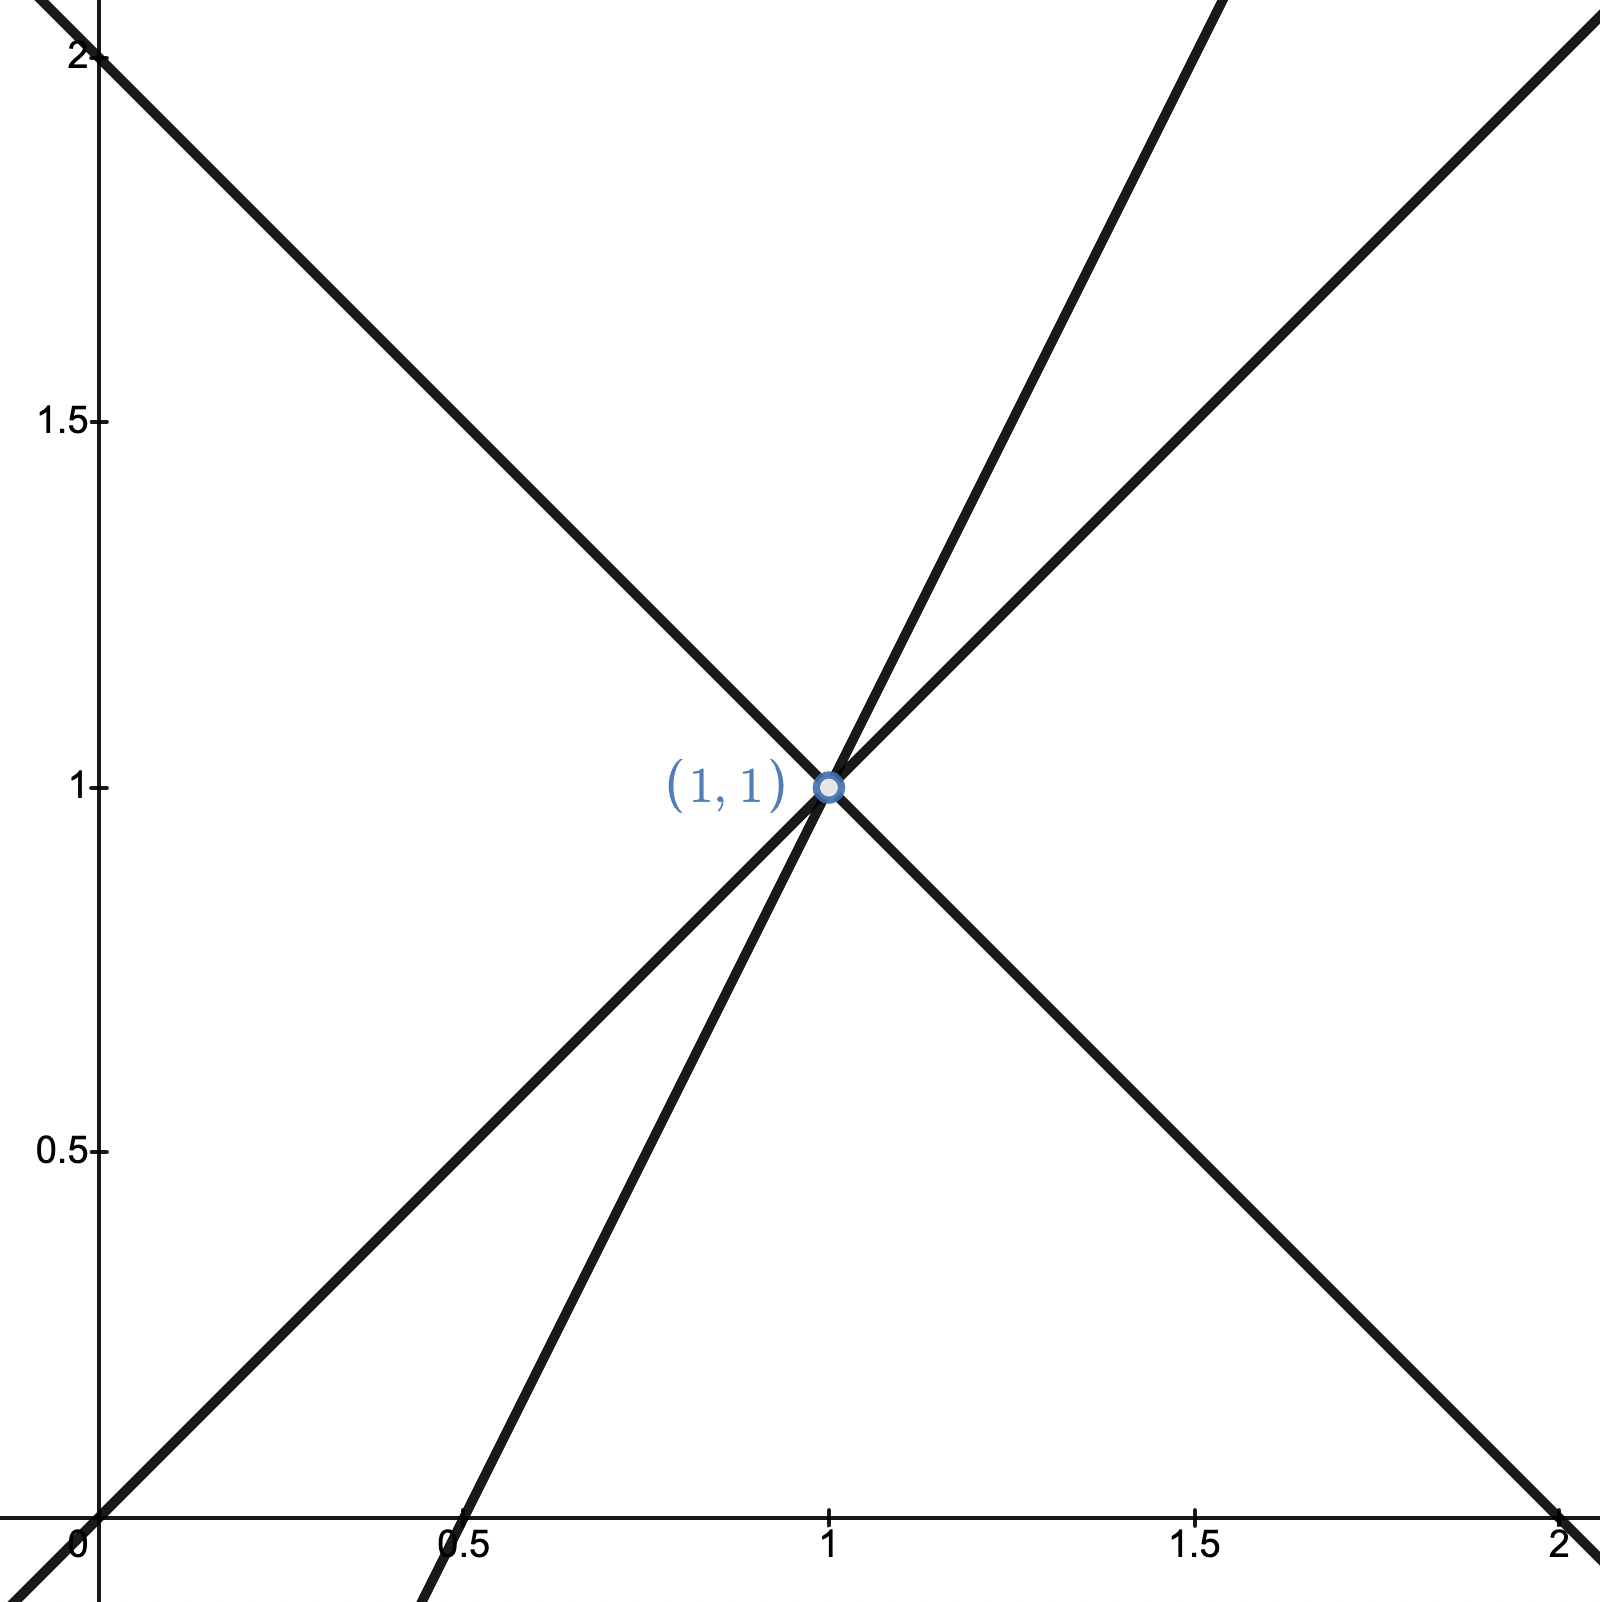
\includegraphics[height=0.333\columnwidth, width=0.5\columnwidth]{lectures/images/definite_system.png}
        \caption*{\scriptsize{Example of definite system.}}
        \label{fig:definite_system}
    \end{wrapfigure}
    Consider a system of the form:
    \[
        \left\{
            \begin{array}{l}
                2x+y = 3,\\
                x+2y = 3,\\
                x-y = 0.
            \end{array}
        \right.  
    \]
    It is obviously that system have only one correct solution in the point $A$ and it is a solution of a type: $\hat{x} = \begin{bmatrix}
        1\\ 1
    \end{bmatrix}$. However, we would like to generalize the method of obtaining a solution in such a way that it looks similar to the first (zero) case, namely:
    \[
        \hat{x} = ?\cdot \vec{b}.  
    \]

    And looking ahead we can obtain such a factor to express solution that way. But now let's get a broader generalization.
    \begin{itemize}
        \item[2. ] Also we can obtain an indefinite solution, that can provide us an infinite amount of solutions.
    \end{itemize}

    \begin{wrapfigure}[12]{r}{0.5\columnwidth}
        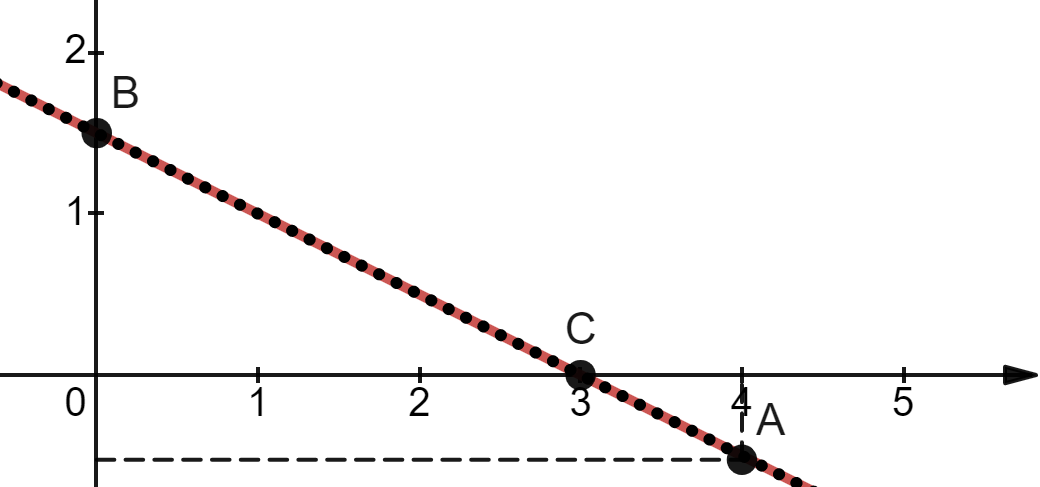
\includegraphics[height=0.235\columnwidth, width=0.5\columnwidth]{lectures/images/indefinite_system.png}
        \caption*{\scriptsize{Example of definite system.}}
        \label{fig:indefinite_system_1}
    \end{wrapfigure}
    Consider a system of two equations:
    \[
        \left\{
            \begin{array}{l}
                x+2y=3,\\
                2x+4y = 5.
            \end{array}
        \right.  
    \]

    It is not so obvious to choose a specific solution here because a whole family of solutions of the following form $\hat{x} = \begin{bmatrix}
        3-2y\\y
    \end{bmatrix}$ is suitable for us. 
    \par 
    And now we need to get some understanding about which solution is a kind of optimum. We will discuss it a little bit later, now let's consider one more possible situation.
    \begin{itemize}
        \item[3. ] 
    \end{itemize}

    \begin{wrapfigure}[18]{r}{0.4\columnwidth}
        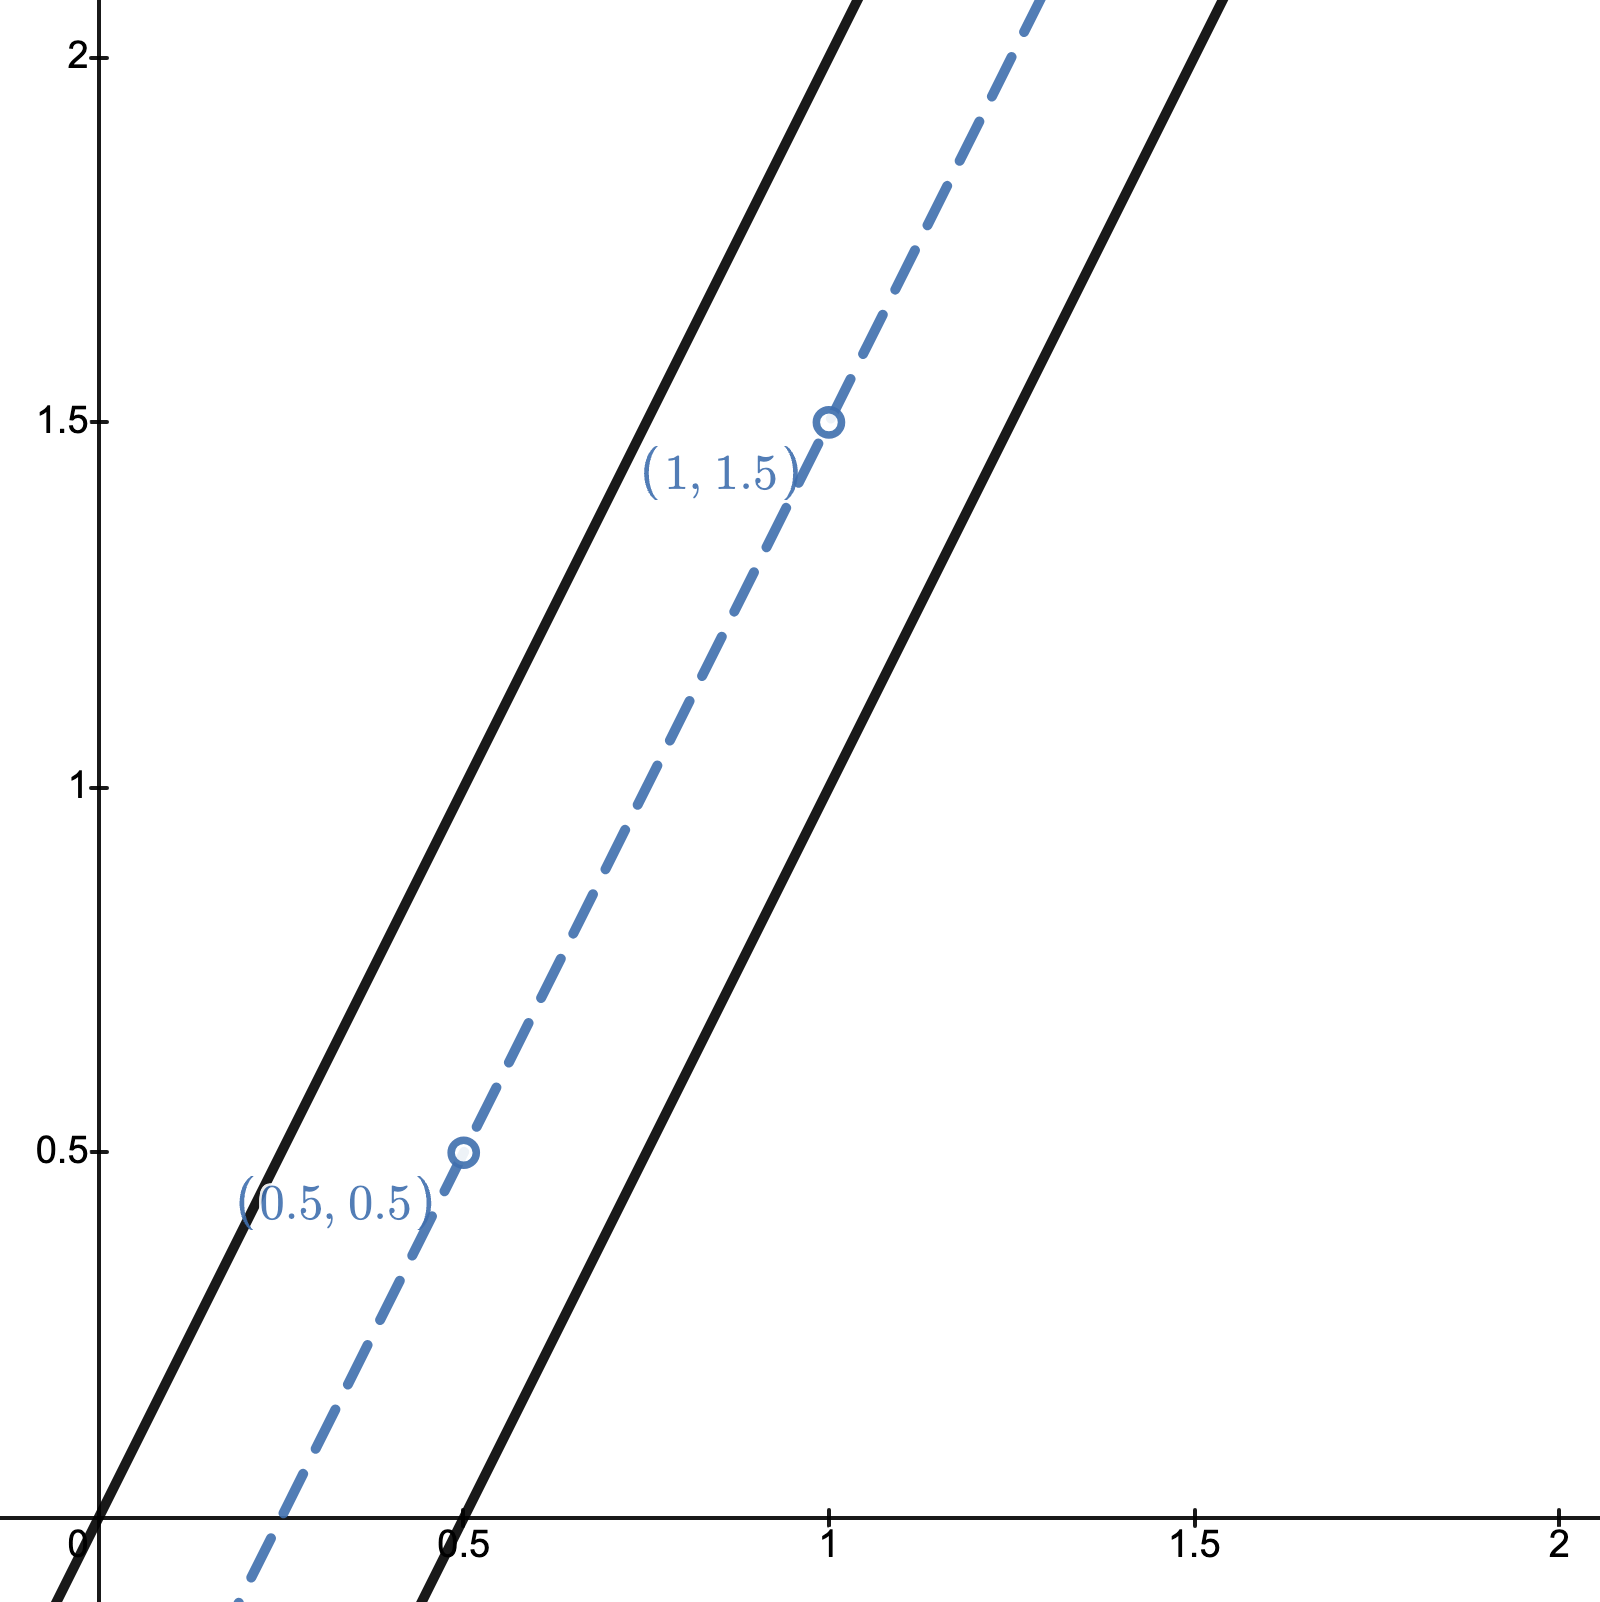
\includegraphics[height=0.45\columnwidth, width=0.36\columnwidth]{lectures/images/inconsistent_system.png}
        \caption*{\scriptsize{Example of inconsistent system.}}
        \label{fig:inconsistent_with_vectors}
    \end{wrapfigure}
    Inconsistent system is a system of a kind:
        \[
            \left\{
                \begin{array}{c}
                    2x+y=3,\\
                    2x+y=6
                \end{array}
            \right.  
        \]
    Need to remind, that we want to obtain solution in term of factors:
    \[
         \hat{x} = ? \cdot \vec{b}.
    \]
    There we have matrix and vector of initial values \[A = \begin{bmatrix}
        2 & 1\\
        2 & 1
    \end{bmatrix} \ \text{ and }\ \vec{b} = \begin{bmatrix}
        3 \\ 6
    \end{bmatrix}.\] 
    Manually we can understand that the best solution will lie somewhere between two parallel lines, perhaps even exactly in the middle. But it is still a whole family of solutions that can be the answer to the request of the product or business problem. We need a general variant to find the best solution. For this we introduce the definition:
    \par
    \begin{definition}{}{}
        Consider a system of a linear equations $A\vec{x} = \vec{b} \ \left(A \in M_{m\times n}(\C)\right)$. A vector $\vec{u} \in \C^n$ is called a pseudosolution or a least square solution, if $\forall \vec{x} \in \C^n$ the length of $A\vec{u} - \vec{b}$ is less or equal to the length of $A\vec{x} - \vec{b}$:
        \[
            \left| A\vec{u} - \vec{b} \right| \leq \left| A\vec{x} - \vec{b} \right|. 
        \]
        That is: if $f_x = \begin{bmatrix}
            f_1 \\
            \vdots\\
            f_n
        \end{bmatrix} = A\vec{x}-\vec{b}$, then $|f_x|^2 = |f_1|^2 + \ldots + |f_n|^2$ for $\vec{x}=\vec{u}$ is minimal.
    \end{definition}
    \begin{theorema}{}{}
        The vector $\vec{u} = A^+\vec{b}$ is a pseudosolution of the system of linear equations $A\vec{x} = \vec{b}$. Moreover, among all pseudosolutions, $\vec{u}$ has the minimal length.
    \end{theorema}
    \begin{proposition}{}{}
        If $\hat{x}$ is a solution, then it is a pseudosolution.
    \end{proposition}
    \begin{proof}
        $A\hat{x} - \vec{b} = 0 \Longrightarrow \left| A\hat{x} - \vec{b} \right| = 0 = \min |f_x|^2.$
    \end{proof}
    \vspace*{0.2cm}

    \Ex 
    \begin{center}
        \begin{tabular}{|c|c|}
            \hline
            Type of a system & Solution \\ \hline
            definite         &      $\vec{u} = \hat{x}$  is the solution  \\ \hline
            indefinite       &   $\vec{u} = \hat{x}$  is the solution of minimal length       \\ \hline
            inconsistent     &    $\vec{u} = \hat{x}$  is the pseudosolution  of minimal length    \\ \hline
            \end{tabular}
    \end{center}
    \begin{proof} (Of the theorem) In proof we will use
        \begin{theorema}{(Pythagoras)}{}
            Suppose $\vec{a} \perp \vec{b}$, that is $(\vec{a}, \vec{b}) = 0$. Then for $\vec{c} = \vec{a} + \vec{b}: \ |\vec{c}|^2 = |\vec{a}|^2 + |\vec{b}|^2.$ In particular $|\vec{c}| \geq |\vec{a}|$. The equality holds only for $\vec{b} = \vec{0}$.
        \end{theorema}        
        \begin{lemma}{}{}
            $\im A \perp \im B$, where $B = AA^+-I$.
        \end{lemma}
\begin{proof}    
        \begin{wrapfigure}[20]{l}{0.3\columnwidth}
        \tikzset{every picture/.style={line width=1pt}} %set default line width to 0.75pt        
        \hspace*{1.5cm} \scalebox{1.25}{\begin{tikzpicture}[x=0.75pt,y=0.75pt,yscale=-1,xscale=1]
        %uncomment if require: \path (0,300); %set diagram left start at 0, and has height of 300

        %Shape: Circle [id:dp6605284406961527] 
        \draw   (100,122.75) .. controls (100,91.68) and (125.18,66.5) .. (156.25,66.5) .. controls (187.32,66.5) and (212.5,91.68) .. (212.5,122.75) .. controls (212.5,153.82) and (187.32,179) .. (156.25,179) .. controls (125.18,179) and (100,153.82) .. (100,122.75) -- cycle ;
        %Shape: Polygon [id:ds7845026568435469] 
        \draw  [pattern=_xen0kut1n,pattern size=6pt,pattern thickness=1pt,pattern radius=0pt, pattern color={rgb, 255:red, 0; green, 0; blue, 0}] (177.79,102.82) -- (204.29,125.82) -- (154.5,166.57) -- (124.5,146.57) -- cycle ;
        %Shape: Diamond [id:dp1953817249032601] 
        \draw  [pattern=_vilei2kdf,pattern size=6pt,pattern thickness=1pt,pattern radius=0pt, pattern color={rgb, 255:red, 0; green, 0; blue, 0}] (128.07,80.42) -- (162.82,98.03) -- (161.31,136.96) -- (126.57,119.35) -- cycle ;
        % Text Node
        \draw (175.5,83.37) node [anchor=north west][inner sep=0.75pt]   [align=left] {$\displaystyle \mathbb{C}^{n}$};
        % Text Node
        \draw (169.62,157.24) node [anchor=north west][inner sep=0.75pt]  [rotate=-320] [align=left] {$\displaystyle \im A$};
        % Text Node
        \draw (136,69.37) node [anchor=north west][inner sep=0.75pt]   [align=left] {$\displaystyle \im B$};
        \end{tikzpicture}}
\end{wrapfigure} 

We should prove: each column $A^j$ of $A$ is orthogonal to the one $B^l$ of B.
\begin{gather*}
    \text{OR: } \forall l \ \left(B^l, A^j\right) \overset{?}{=} 0, \ \text{ or }\ B^{l^*}\cdot A^j  \overset{?}{=} 0, \\
    \text{or } \ (B^*)_l \cdot A^j \overset{?}{=} 0,\ \text{ or } \ B^*A \overset{?}{=} 0. \\
    \left(\left(AA^+\right)^* - I^*\right)A = \left(AA^+ - I\right)A = AA^+A - A = 0.
\end{gather*}
\end{proof}
\par
\begin{wrapfigure}[3]{r}{0.2\columnwidth}
    \scalebox{2}{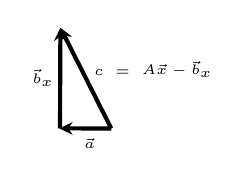
\begin{tikzpicture}[x=0.75pt,y=0.75pt,yscale=-1,xscale=1]
        %uncomment if require: \path (0,300); %set diagram left start at 0, and has height of 300
        
        %Straight Lines [id:da6378479454727755] 
        \draw [line width=1.5]    (104,139.98) -- (125,140) ;
        \draw [shift={(100,139.97)}, rotate = 0.07] [fill={rgb, 255:red, 0; green, 0; blue, 0 }  ][line width=0.08]  [draw opacity=0] (6.43,-3.09) -- (0,0) -- (6.43,3.09) -- (4.27,0) -- cycle    ;
        %Straight Lines [id:da9894819462343878] 
        \draw [line width=1.5]    (100.31,139.97) -- (100.48,95.5) ;
        \draw [shift={(100.5,91.5)}, rotate = 90.22] [fill={rgb, 255:red, 0; green, 0; blue, 0 }  ][line width=0.08]  [draw opacity=0] (6.43,-3.09) -- (0,0) -- (6.43,3.09) -- (4.27,0) -- cycle    ;
        %Straight Lines [id:da5418126690660368] 
        \draw [line width=1.5]    (125,140) -- (102.3,95.07) ;
        \draw [shift={(100.5,91.5)}, rotate = 63.2] [fill={rgb, 255:red, 0; green, 0; blue, 0 }  ][line width=0.08]  [draw opacity=0] (6.43,-3.09) -- (0,0) -- (6.43,3.09) -- (4.27,0) -- cycle    ;
        
        % Text Node
        \draw (115.19,106.07) node [anchor=north west][inner sep=0.75pt]  [font=\tiny,rotate=-359.85] [align=left] {$\displaystyle c\ =\ A\vec{x} -\vec{b}_{x}$};
        % Text Node
        \draw (110.4,143.4) node [anchor=north west][inner sep=0.75pt]  [font=\tiny] [align=left] {$\displaystyle \vec{a}$};
        % Text Node
        \draw (85.4,110) node [anchor=north west][inner sep=0.75pt]  [font=\tiny] [align=left] {$\displaystyle \vec{b}_{x}$};
        \end{tikzpicture}}
\end{wrapfigure}    
We need to prove that $\vec{u}$ is a pseudosolution. Let $\vec{x} \in \C^n$. We need to show:
\[
    \left| A\vec{x} = \vec{b} \right| \geq \left| A\vec{u} - \vec{b}\right|. 
\]

Here $\vec{c} = A\vec{x} - \vec{b} = A\vec{x} - A\vec{u} + A\vec{u} - \vec{b} = A(\vec{x} - \vec{u}) + AA^+\vec{b} - \vec{b} = \\ \hspace*{4.5cm} = A(\vec{x} - \vec{u}) + (AA^+-I)\vec{b} = \underbrace{A\left(\vec{x} - \vec{u}\right)}_{\vec{b}_x} + \underbrace{B\vec{b}}_{\vec{a}}$.
\par 
By Lemma, $\vec{b}_x \perp \vec{a}$. By Pythagoras theorem, $|\vec{c}| = \min \Longleftrightarrow \vec{b}_x = \vec{0}$. For example, it is so for $\vec{x} = \vec{u}$. So $\vec{u}$ is a pseudosolution.
\par
We have shown, what $\vec{x}$ is a pseudosolution $\Longleftrightarrow \vec{b}_x = 0$ or $A(\vec{x} - \vec{u}) = 0$, or $A\vec{x} = A\vec{u}$, or $A\vec{x} = AA^+\vec{b}$. 
\par
Suppose $\vec{x}$ is another pseudosolution. We need to prove that $|\vec{u}| \leq |\vec{x}|$. Let $\vec{w} = \vec{x} - \vec{u}$.
\par
\begin{wrapfigure}[10]{l}{0.2\columnwidth}
    \hspace*{1.5cm} \scalebox{2}{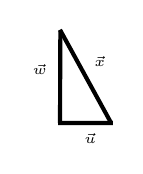
\begin{tikzpicture}[x=0.75pt,y=0.75pt,yscale=-1,xscale=1]
        %uncomment if require: \path (0,300); %set diagram left start at 0, and has height of 300
        
        %Straight Lines [id:da6378479454727755] 
        \draw [line width=1.5]    (99.45,139.98) -- (125.74,140) ;
       %Straight Lines [id:da9894819462343878] 
        \draw [line width=1.5]    (100.31,139.97) -- (100.48,95.5) ;
        %Straight Lines [id:da5418126690660368] 
        \draw [line width=1.5]    (124.95,140) -- (100.3,95.07) ;
        
        % Text Node
        \draw (115.19,106.07) node [anchor=north west][inner sep=0.75pt]  [font=\tiny,rotate=-359.85] [align=left] {$\displaystyle \vec{x}$};
        % Text Node
        \draw (110.4,143.4) node [anchor=north west][inner sep=0.75pt]  [font=\tiny] [align=left] {$\displaystyle \vec{u}$};
        % Text Node
        \draw (85.4,110) node [anchor=north west][inner sep=0.75pt]  [font=\tiny] [align=left] {$\displaystyle \vec{w}$};
        \end{tikzpicture}}
\end{wrapfigure} 
If we prove that $\vec{w}\perp \vec{u}$ then $|\vec{x}| \geq |\vec{u}|$. We have 
\[
  \left(\vec{u}, \vec{w}\right) = \vec{u}^* \vec{w} = (A^+\vec{b})^* \vec{w} = b^*A^{+^*} \vec{w}, \ \text{ where }\ A\vec{w} = 0
\]
\par
Here $(A^+)* \overset{\rom{2}}{=} \left(A^+AA^+\right)^* = A^{+^*}\left(A^+A\right)^* \overset{\rom{4}}{=} A^{+^*}A^+A$. So 
\[(\vec{u}, \vec{w}) = b^*A^{+^*}A^+\underbrace{A\vec{w}}_{0} = 0.\]
\end{proof}
\par
Let's return to our inconsistent system and find pseudosolution:
\[
    A = \begin{bmatrix}
        2 & 1\\
        2 & 1
    \end{bmatrix}, \hspace*{0.5cm} \vec{b} = \begin{bmatrix}
        3 \\ 6
    \end{bmatrix}  
\]

Then pseudosolution can be found by the formula:
\[
    \hat{x} = A^+\vec{b}.  
\]

Pseudoinverse matrix to $A$ can be obtained by:
\begin{gather*}
    A^+ = \left( \begin{bmatrix}
        1 \\ 1
    \end{bmatrix} \cdot \begin{bmatrix}
        2 & 1
    \end{bmatrix}\right)^+ = \begin{bmatrix}
        2 & 1
    \end{bmatrix}^+ \cdot \begin{bmatrix}
        1 \\ 1
    \end{bmatrix}^+ = \dfrac{1}{2}\cdot\dfrac{1}{5} \begin{bmatrix}
        2 & 2 \\
        1 & 1
    \end{bmatrix} = \dfrac{1}{10} \begin{bmatrix}
        2 & 2 \\
        1 & 1
    \end{bmatrix}
\end{gather*}

Then we can get a pseudosolution:
\[
    \hat{x} = \dfrac{1}{10} \begin{bmatrix}
        2 & 2 \\
        1 & 1
    \end{bmatrix} \cdot \begin{bmatrix}
        3 \\ 
        6
    \end{bmatrix} = \dfrac{1}{10} \begin{bmatrix}
        18 & 9
    \end{bmatrix}
\]
\begin{proposition}{}{}
    $\vec{x}\ $ is a pseudosolution $\Longleftrightarrow \vec{x}\ $ is a solution of the "normal" system of a kind:
    \[
        A^*A\vec{x} = A^*\vec{b}.  
    \]
\end{proposition}

\begin{proposition}{}{}
    All pseudosolutions (solutions) of $A\vec{x} = \vec{b}$ are given by the formula:
    \[
        \vec{x} = A^+\vec{b} - (A^+A-I)\vec{y},  
    \]
    where $\vec{y} \in \C^n$ -- orbitary vector.
\end{proposition}

Now let's find all pseudosolutions for example with inconsistent system. We have already obtained one pseudosolution:
\[
    \hat{x} = \dfrac{1}{10}\begin{bmatrix}
        18\\
        9
    \end{bmatrix}  
\]

Now we need to obtain $A^+A-I$:
\[
    A^+A-I = \dfrac{1}{10} \begin{bmatrix}
        2 & 2 \\
        1 & 1
    \end{bmatrix} \cdot \begin{bmatrix}
        2 & 1\\
        2 & 1
    \end{bmatrix} - \begin{bmatrix}
        1 & 0\\
        0 & 1
    \end{bmatrix} = \dfrac{1}{10}\begin{bmatrix}
        8 & 4 \\
        4 & 2
    \end{bmatrix} - \begin{bmatrix}
        1 & 0 \\
        0 & 1
    \end{bmatrix} = \begin{bmatrix}
        -0.2 & 0.4 \\
        0.4 & -0.8
    \end{bmatrix}
\]

Finally,
\[
    \hat{x} = \dfrac{1}{10}\begin{bmatrix}
        18 \\ 9
    \end{bmatrix} - \begin{bmatrix}
        -0.2 & 0.4\\
        0.4 & -0.8
    \end{bmatrix}  \begin{bmatrix}
        y_1 \\
        y_2
    \end{bmatrix} = \begin{bmatrix}
        1.8 + 0.2y_1 - 0.4 y_2\\
        0.9 - 0.4y_1 + 0.8y_2
    \end{bmatrix} 
\]
\subsection*{Linear regression problem}


\begin{wrapfigure}{l}{1\columnwidth}
    \scalebox{1.5}{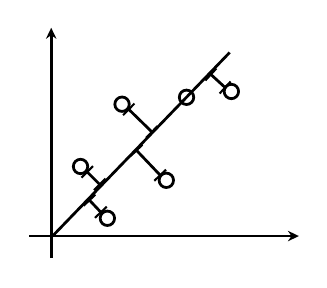
\begin{tikzpicture}[x=0.75pt,y=0.75pt,yscale=-1,xscale=1]
        %uncomment if require: \path (0,300); %set diagram left start at 0, and has height of 300
        
        %Straight Lines [id:da021044538065793983] 
        \draw    (100.4,150.71) -- (100.4,42.71) ;
        \draw [shift={(100.4,39.71)}, rotate = 90] [fill={rgb, 255:red, 0; green, 0; blue, 0 }  ][line width=0.08]  [draw opacity=0] (5.36,-2.57) -- (0,0) -- (5.36,2.57) -- (3.56,0) -- cycle    ;
        %Straight Lines [id:da768552366016573] 
        \draw    (89.73,140.05) -- (216.73,140.05) ;
        \draw [shift={(219.73,140.05)}, rotate = 180] [fill={rgb, 255:red, 0; green, 0; blue, 0 }  ][line width=0.08]  [draw opacity=0] (5.36,-2.57) -- (0,0) -- (5.36,2.57) -- (3.56,0) -- cycle    ;
        %Shape: Circle [id:dp4077752415315412] 
        \draw   (111.06,106.53) .. controls (111.06,104.62) and (112.62,103.06) .. (114.53,103.06) .. controls (116.45,103.06) and (118,104.62) .. (118,106.53) .. controls (118,108.45) and (116.45,110) .. (114.53,110) .. controls (112.62,110) and (111.06,108.45) .. (111.06,106.53) -- cycle ;
        %Shape: Circle [id:dp2037573912425814] 
        \draw   (123.99,131.49) .. controls (123.99,129.57) and (125.55,128.02) .. (127.46,128.02) .. controls (129.38,128.02) and (130.93,129.57) .. (130.93,131.49) .. controls (130.93,133.4) and (129.38,134.96) .. (127.46,134.96) .. controls (125.55,134.96) and (123.99,133.4) .. (123.99,131.49) -- cycle ;
        %Shape: Circle [id:dp45400412163463866] 
        \draw   (162.13,73.2) .. controls (162.13,71.28) and (163.68,69.73) .. (165.6,69.73) .. controls (167.51,69.73) and (169.07,71.28) .. (169.07,73.2) .. controls (169.07,75.11) and (167.51,76.67) .. (165.6,76.67) .. controls (163.68,76.67) and (162.13,75.11) .. (162.13,73.2) -- cycle ;
        %Shape: Circle [id:dp5342492536064438] 
        \draw   (131.06,76.53) .. controls (131.06,74.62) and (132.62,73.06) .. (134.53,73.06) .. controls (136.45,73.06) and (138,74.62) .. (138,76.53) .. controls (138,78.45) and (136.45,80) .. (134.53,80) .. controls (132.62,80) and (131.06,78.45) .. (131.06,76.53) -- cycle ;
        %Shape: Circle [id:dp2972731544634346] 
        \draw   (152.4,113.2) .. controls (152.4,111.28) and (153.95,109.73) .. (155.87,109.73) .. controls (157.78,109.73) and (159.33,111.28) .. (159.33,113.2) .. controls (159.33,115.11) and (157.78,116.67) .. (155.87,116.67) .. controls (153.95,116.67) and (152.4,115.11) .. (152.4,113.2) -- cycle ;
        %Straight Lines [id:da2595807846962981] 
        \draw    (101.06,140.05) -- (186.4,51.6) ;
        %Shape: Circle [id:dp7278044041658378] 
        \draw   (183.73,70.4) .. controls (183.73,68.48) and (185.28,66.93) .. (187.2,66.93) .. controls (189.11,66.93) and (190.67,68.48) .. (190.67,70.4) .. controls (190.67,72.31) and (189.11,73.87) .. (187.2,73.87) .. controls (185.28,73.87) and (183.73,72.31) .. (183.73,70.4) -- cycle ;
        %Straight Lines [id:da4346572573275653] 
        \draw    (117.75,109.16) -- (123.75,115.16) ;
        \draw [shift={(123.75,115.16)}, rotate = 225] [color={rgb, 255:red, 0; green, 0; blue, 0 }  ][line width=0.75]    (0,3.91) -- (0,-3.91)   ;
        \draw [shift={(117.75,109.16)}, rotate = 225] [color={rgb, 255:red, 0; green, 0; blue, 0 }  ][line width=0.75]    (0,3.91) -- (0,-3.91)   ;
        %Straight Lines [id:da18387194843836618] 
        \draw    (124.32,128.59) -- (118.84,122.78) ;
        \draw [shift={(118.84,122.78)}, rotate = 46.7] [color={rgb, 255:red, 0; green, 0; blue, 0 }  ][line width=0.75]    (0,3.91) -- (0,-3.91)   ;
        \draw [shift={(124.32,128.59)}, rotate = 46.7] [color={rgb, 255:red, 0; green, 0; blue, 0 }  ][line width=0.75]    (0,3.91) -- (0,-3.91)   ;
        %Straight Lines [id:da2364994210811795] 
        \draw    (137.76,79.01) -- (148.9,89.87) ;
        \draw [shift={(148.9,89.87)}, rotate = 224.26] [color={rgb, 255:red, 0; green, 0; blue, 0 }  ][line width=0.75]    (0,3.91) -- (0,-3.91)   ;
        \draw [shift={(137.76,79.01)}, rotate = 224.26] [color={rgb, 255:red, 0; green, 0; blue, 0 }  ][line width=0.75]    (0,3.91) -- (0,-3.91)   ;
        %Straight Lines [id:da8931600019469914] 
        \draw    (141.51,98.78) -- (152.9,110.73) ;
        \draw [shift={(152.9,110.73)}, rotate = 226.36] [color={rgb, 255:red, 0; green, 0; blue, 0 }  ][line width=0.75]    (0,3.91) -- (0,-3.91)   ;
        \draw [shift={(141.51,98.78)}, rotate = 226.36] [color={rgb, 255:red, 0; green, 0; blue, 0 }  ][line width=0.75]    (0,3.91) -- (0,-3.91)   ;
        %Straight Lines [id:da2901806653749395] 
        \draw    (177.33,62.2) -- (184.19,68.49) ;
        \draw [shift={(184.19,68.49)}, rotate = 222.51] [color={rgb, 255:red, 0; green, 0; blue, 0 }  ][line width=0.75]    (0,3.91) -- (0,-3.91)   ;
        \draw [shift={(177.33,62.2)}, rotate = 222.51] [color={rgb, 255:red, 0; green, 0; blue, 0 }  ][line width=0.75]    (0,3.91) -- (0,-3.91)   ;
        \end{tikzpicture}}
\end{wrapfigure} 
